\documentclass[12pt,letter]{article}

\usepackage[T1]{fontenc}
\usepackage[utf8]{inputenc}
\usepackage{lmodern}

\usepackage[english]{babel}
\usepackage{csquotes}

\usepackage[authordate,backend=biber]{biblatex-chicago}

\bibliography{../library}

\usepackage{amssymb,amsmath,amsfonts,eurosym,float,geometry,multirow,ulem,graphicx,caption,color,setspace,sectsty,comment,footmisc,caption,pdflscape,subfig,array,hyperref,outlines,placeins}

\normalem

\newtheorem{theorem}{Theorem}
\newtheorem{corollary}[theorem]{Corollary}
\newtheorem{proposition}{Proposition}
\newenvironment{proof}[1][Proof]{\noindent\textbf{#1.} }{\ \rule{0.5em}{0.5em}}

\newtheorem{hyp}{Hypothesis}
\newtheorem{subhyp}{Hypothesis}[hyp]
\renewcommand{\thesubhyp}{\thehyp\alph{subhyp}}

\newcommand{\red}[1]{{\color{red} #1}}
\newcommand{\blue}[1]{{\color{blue} #1}}

\newcolumntype{L}[1]{>{\raggedright\let\newline\\arraybackslash\hspace{0pt}}m{#1}}
\newcolumntype{C}[1]{>{\centering\let\newline\\arraybackslash\hspace{0pt}}m{#1}}
\newcolumntype{R}[1]{>{\raggedleft\let\newline\\arraybackslash\hspace{0pt}}m{#1}}

\geometry{left=1.0in,right=1.0in,top=1.0in,bottom=1.0in}


\begin{document}

\setcounter{page}{1}

\title{\Large Does Franchise Expansion Affect Legislative Activity?:\\ Evidence from British India Legislative Debates, 1916-1925}
\author{Mitchell Bosley\thanks{PhD Candidate, Department of Political Science, University of Michigan. e-mail: mcbosley@umich.edu} and Htet Thiha Zaw\thanks{PhD Candidate, Department of Political Science, University of Michigan. e-mail: htzaw@umich.edu}}
\date{\today}
\maketitle
\begin{abstract}
\noindent Universal suffrage, the unconditional provision of voting rights for every adult citizen, is a key element of democracy. The transition from a more limited to less limited franchise, therefore, is purported to bring diverse policy preferences to the legislature. While existing research has identified such transformation by looking at policy outcomes, it lacks an explanation of how they were brought about in the legislature, a key actor in policy formation. We fill this gap with the first-ever text-as-data analysis of the British India legislature for ten years between 1916 and 1925, showing the impact of franchise expansion in 1920. Contrary to our expectations, we do not find that policy preferences are significantly different between elected and non-elected members overall. Instead, we observe divergence from the unelected members by only some subgroups of the new elected members. The findings will provide a new perspective on colonial legislatures and their role in policy formation after franchise expansion.\\
%\noindent\textbf{JEL Codes:} key1, key2, key3\\

\end{abstract}

\doublespacing

\section{Motivation}
How did governments form policies in colonial states? While existing historical political economy research highlights the many policy decisions made under colonial rule as well as their consequences for state development, the institutions in place for creating them remain poorly understood beyond individual historical accounts. Particularly, the role that colonial legislative institutions, which initially emerged in North America and then later spread to colonies across Africa and Asia, play in policy formation has only recently received attention \parencite{gailmardBuildingNewImperial2017,paineDemocraticContradictionsEuropean2019}.

In this paper, we analyze one key feature of the policy-making process: the ideology of the legislators who craft the policy. We look to the history of British India to show how a key institutional change -- suffrage expansion -- affects the ideological distribution of members of the Indian Legislative Assembly between 1921 and 1926. We argue that, with the introduction of a larger electorate with different policy preferences in the legislature, franchise expansion fundamentally reshaped the role of colonial legislative institutions in policy formation. Specifically, in a legislature where some members are elected and others are not, we expect elected members (who are elected with a broad voter base) to differ ideologically from unelected members.\par

Using ten-thousand speeches from both elected and unelected members of the assembly, we fit a speech-based ideal point estimation model from \textcite{vafaTextBasedIdealPoints2020} and show preliminary evidence that, contrary to our expectations, members of the Legislative Assembly do \textit{not} cluster ideologically based on whether they were elected or not. \par

\section{Historical Context}
% We then look at British India to understand the role of colonial legislative institutions in policy formation, and if franchise expansion can bring substantial changes in its role.
Most territories of present-day India were formally organized as a British crown colony under Government of India Act of 1858, which effectively transferred political administration from the British East India Company to the crown government. Enacted just after a violent rebellion, the law was part of the numerous institutional reforms that followed, one being the establishment of Imperial Legislative Council in 1861. This legislature was mainly composed of nominated members by the governor and elected members from organizations such as Bombay Chamber for Commerce.\par

Following the First World War, the 1919 Government of India Act introduced two key reforms that fundamentally reshaped the Indian Parliament: the bicameral division of the Indian parliament the Imperial Legislative Assembly and Council of States, and the expansion of the electoral franchise to indigenous peoples of British India (subject to gender and property restrictions). After 1919, then, both houses of the Indian Parliament contained appointed (unelected) and elected members. Notably, many elected members were members of the indigenous peoples who had been granted suffrage. Their seats could either be broadly geographic (such as Madras) or sector-specific (e.g., Muslim landholders). Figure \ref{fig:leg_before_after} shows that the expansion resulted in a significant increase in legislature size, from roughly 60 members before 1920 to around 200 members by 1921. The growth mainly came from elected members, which increased from around 20 members to around 130 members, now representing roughly two-third of the legislature.\par

\begin{figure}
    \centering
    \includegraphics[width=\linewidth]{../figs/members.png}
    \caption{Number of colonial legislative members, 1916-1930. Red represents appointed members and blue represents elected members. Figures after 1920 are from both chambers. Data collected by authors.}
    \label{fig:leg_before_after}
\end{figure}

\section{Data and Methods}
To evaluate the effect of suffrage expansion on legislative behavior we create a novel historical data created from the documents covering British India parliamentary debates from 1916 to 1925; this totals nearly 4,000 sessions from both chambers as compiled by India Parliament Digital Library. Figure \ref{fig:example_page} shows one page from a 1921 debate from the Legislative Assembly. Each of these documents contain daily questions and answers as well as debates on various topics in Legislative Assembly and Council of States.

We used the \textit{R} package Tesseract to translate each of these PDF files to plain text, and then used a regular expression script to parse the individual speeches. We have collected 166,000 speeches from the 1918-1921 (pre-reform) Imperial Legislative Council and the 1921-1926 (post-reform) upper and lower houses, and we plan to collect the speeches from 1926 to the present in the same manner. We merge this speech data to a member level data that indicates whether an MP was elected, and if so, what constituency they are elected by (Muslim, non-Muslim, Sikh, Landholders, etc.) For this analysis, we use 10,000 speeches from the lower house during the 1921-1926 period, but plan to expand our analysis to the rest of our dataset in the near future. Figure \ref{fig:descrip_stats} shows the speech and speaker-level breakdown of the data used in this analysis.\par

To estimate the ideological distribution of the members of the Legislative Assembly in our data, we employ the text-based ideal point estimation model from \textcite{vafaTextBasedIdealPoints2020}, which uses a estimate the parameters of the Poisson factorization model
\[y_{dv} \sim \text{Pois}\big(\sum_k \theta_{dk} \beta_{kv} \exp\{x_{a_d}\eta _{kv}\}\big),\]
where \(y_{dv}\) is the word count of vocabulary term \(v\) in document \(d\), \(\theta_{dk}\) is a scalar representing the intensity of the non-ideological part of topic \(k\) in document \(d\), \(\beta_{kv}\) is a scalar representing the frequency of word \(v\) in the non-ideological part of topic \(k\), \(x_{a_d}\) is the scalar ideal point of author \(a\) for document \(d\), and \(\eta_{kv}\) is the scalar representing the frequency of a word \(v\) in the ideological part of the topic. The goal is to estimate the parameters of this model, one of which is the ideal point \(x_{ad}\).\footnote{The high level interpretation of this equation is that for \(k\) topics, the data matrix (a document-term matrix where each row is a document and each column is a count of words) is factorized into matrices \(\theta\), which contains per-document topic intensities, \(\beta\), which contains the non-ideological (i.e., common across speakers) dimension of the topics and \(\eta\), which contains the ideological (i.e., not common across speakers) topics, and \(x\), which is a scalar ideal point for the author that persists across topics.For a more complete description of the model, see section 2.3 in \textcite{vafaTextBasedIdealPoints2020}.} Because of the intractability of this model, the authors recommend using a variational inference algorithm to estimate the model's parameters. We follow this advice, and run the model on Google Colab, a free cloud-based computing service\footnote{For instructions on how to run the model, see \url{https://github.com/keyonvafa/tbip}}.

\begin{figure}
    \centering
    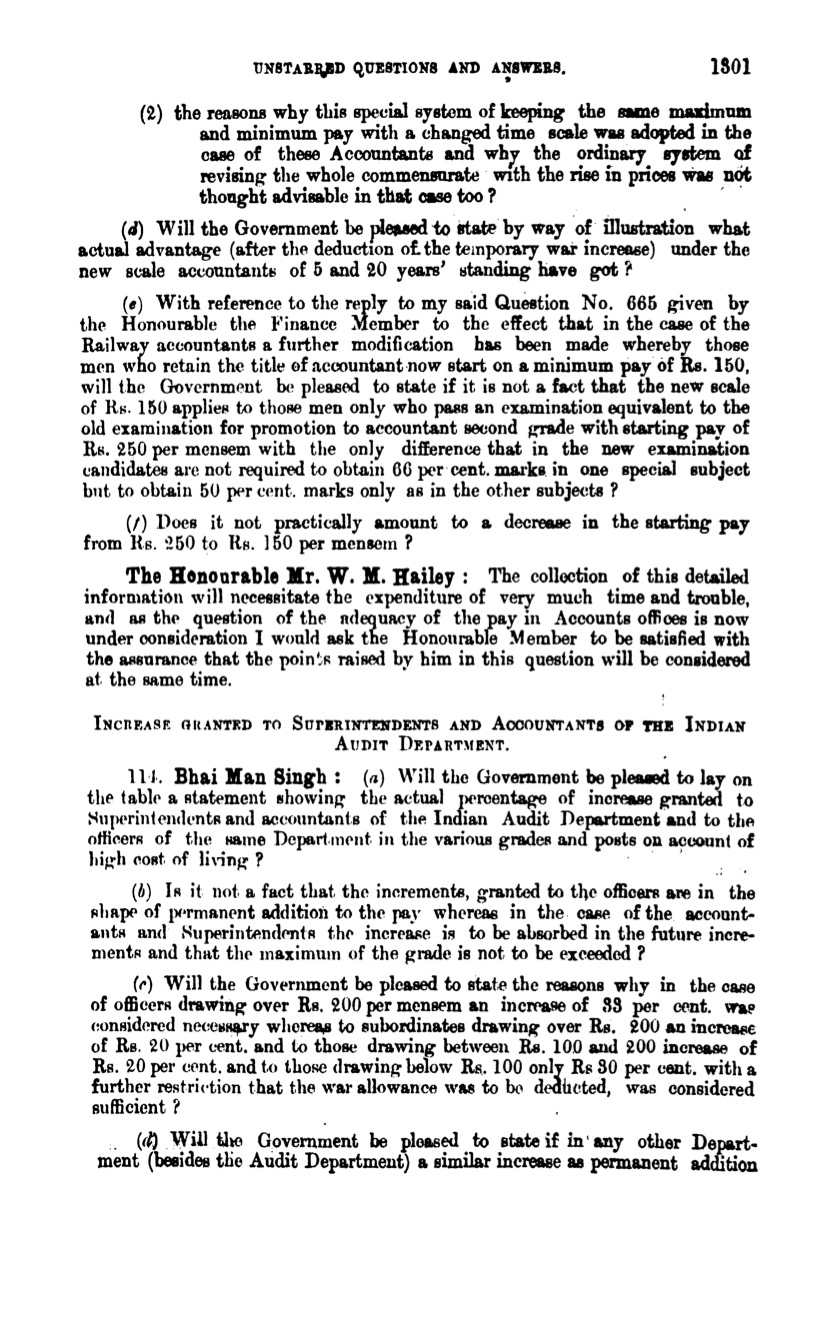
\includegraphics[width=0.85\linewidth]{../figs/example_page.jpg}
    \caption{One Page from the September 30th 1921 debate of the Legislative Assembly.}
    \label{fig:example_page}
\end{figure}

\begin{figure}
    \centering
    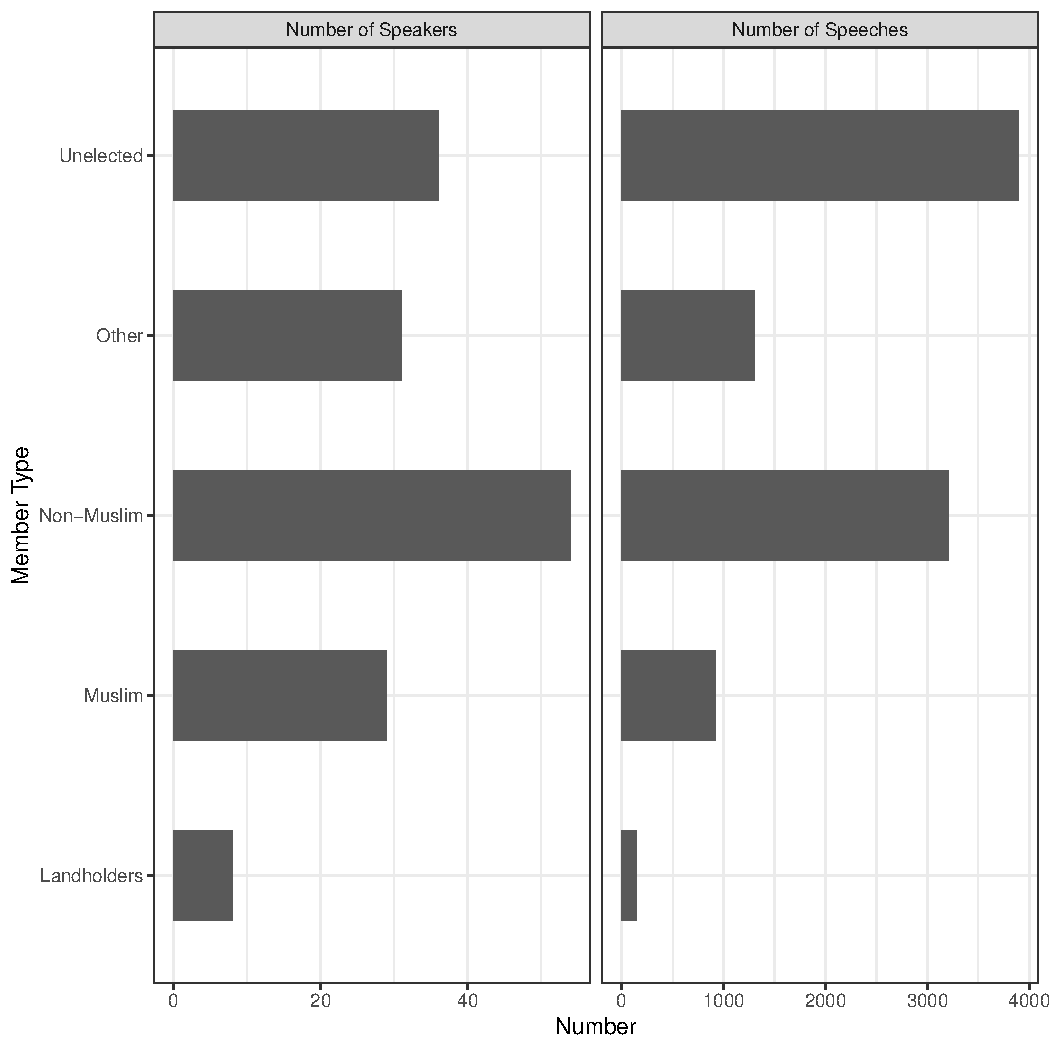
\includegraphics[width=\linewidth]{../figs/speech-speaker-prop.pdf}
    \caption{Breakdown of number of speakers and number of speeches by group type from modeled data.}
    \label{fig:descrip_stats}
\end{figure}

\section{Findings and Discussion}

\begin{figure}
    \centering
    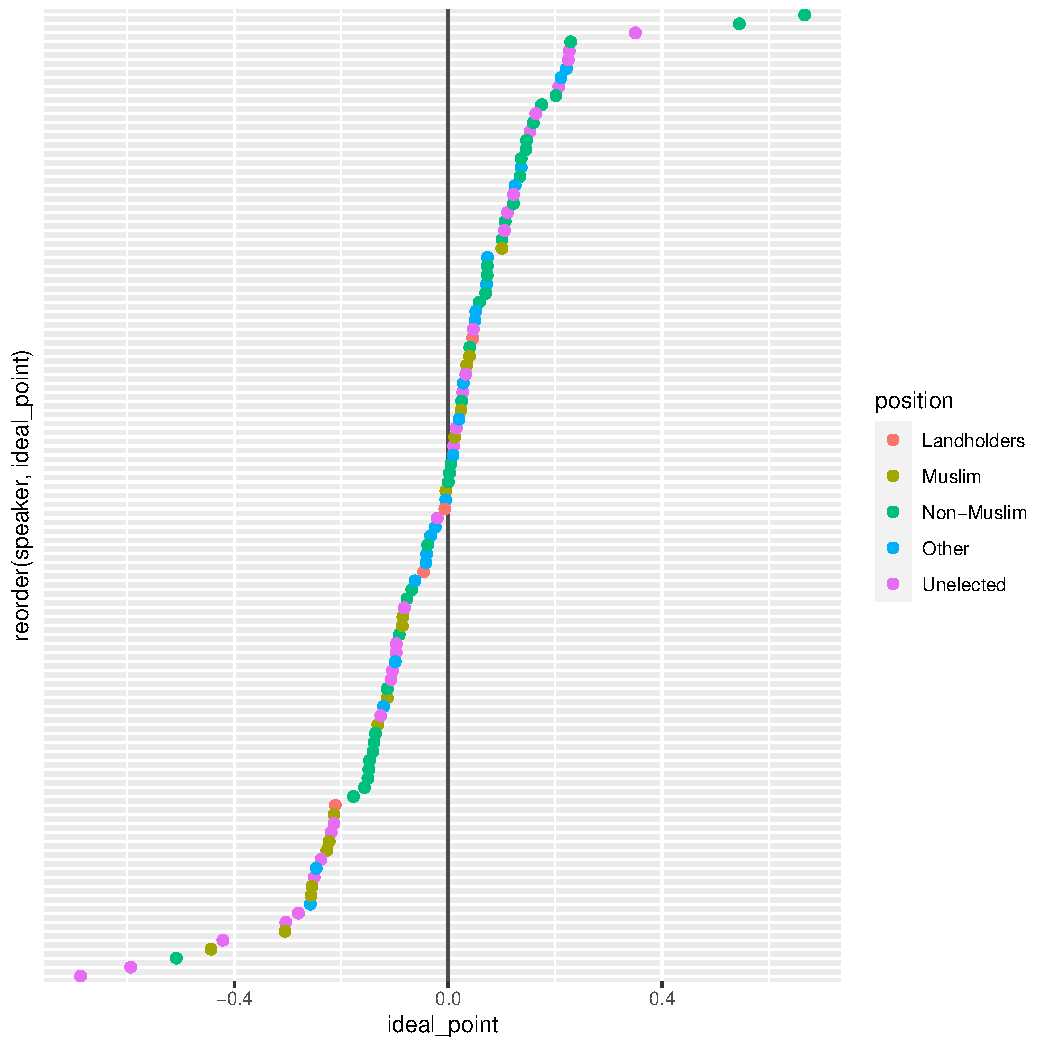
\includegraphics[width=\linewidth]{../figs/pointplot.pdf}
    \caption{Estimated Ideal Points for Each Assembly Member, by Constituency.}
    \label{fig:ideal_points}
\end{figure}

\begin{figure}
    \centering
    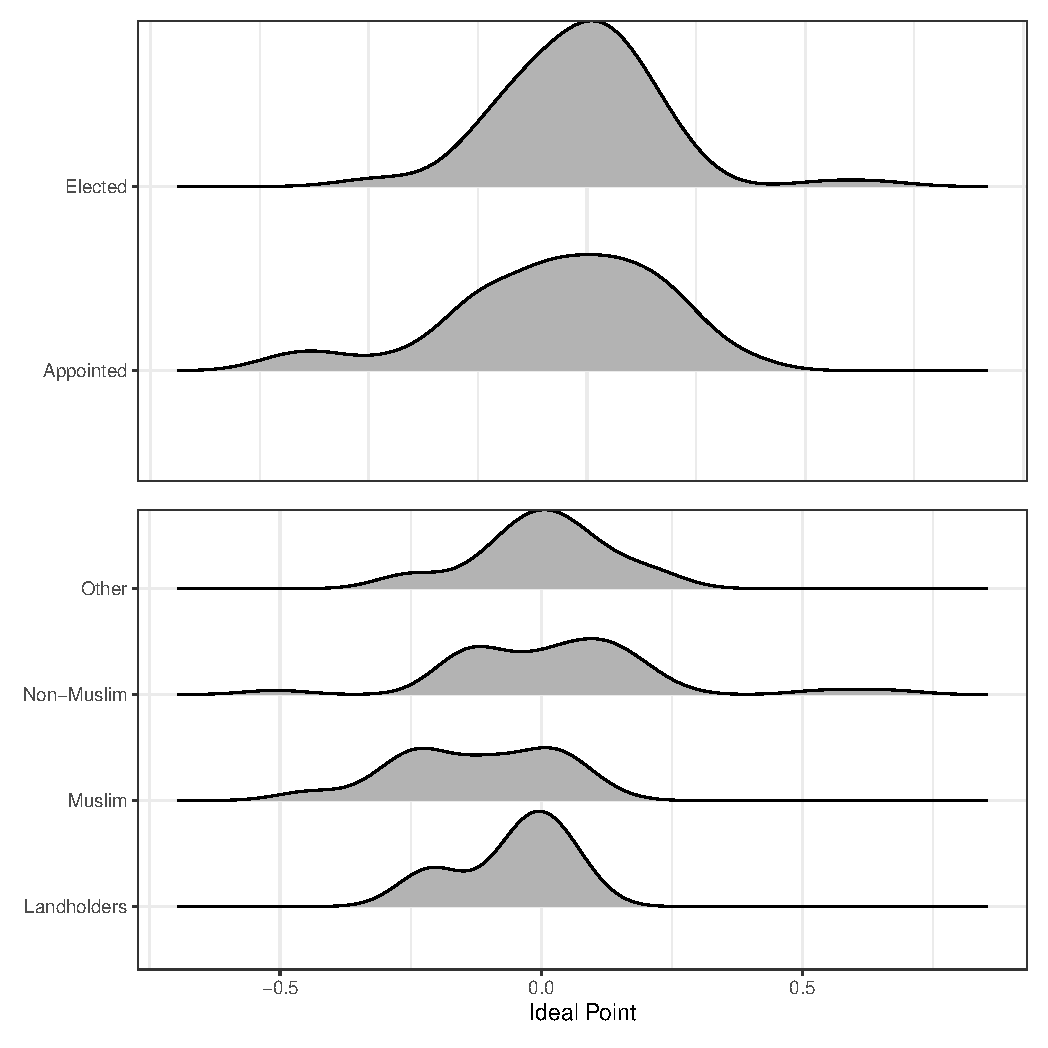
\includegraphics[width=\linewidth]{../figs/ridges_combined.pdf}
    \caption{Distribution of ideal points for elected/unelected members (top) and by constituency type for elected members (bottom).}
    \label{fig:ideal_dist}
\end{figure}

We present our main results in figures \ref{fig:ideal_points}, which shows the ideal points estimated for each of the Assembly members, grouped by constituency, and \ref{fig:ideal_dist}, which shows the distribution of ideal points for elected and unelected (appointed) members, as well as for each sub-group within the elected members.

While we do not observe a difference between elected and unelected members in the aggregate, we do observe a leftward skew to the distribution of ideal points for Muslim elected members, and a rightward skew for for non-Muslim elected members. Our interpretation is that the expected divergence in between elected and unelected members is qualified by demographic group.\footnote{It is important to not read too far into the left-right scale here. The model isn't measuring left-right ideology in the value-laden way that we think about it today. Rather, it's measuring partisan sorting on a single dimension, and is agnostic to the content of that dimension.}

In closing, we would like to emphasize that this is very much a preliminary analysis. We plan to collect more data (in particular, we are interested in adding the party attachment of each of the members) and run other models (e.g., the structural topic model) to explore the data. In particular, we are interested in expanding the model from \textcite{vafaTextBasedIdealPoints2020} in two key ways: first, by introducing a temporal component, so that ideal points can be measured over time; and second, by adding multidimensional ideal points in order to measure the dimensionality of debate over time. Thank-you for taking the time to read this! We welcome any and all feedback.
\par
\newpage
\printbibliography

\end{document}
